\chapter{Neutral Current Spectrum Prediction}
\label{ch:Prediction}

In order to extract measurements of oscillation parameters, the measured FD spectrum must be compared to a predicted distribution. The FD MC by itself does not constitute a good prediction due to various uncertainties like the beam flux and interaction cross sections. A more robust prediction is crafted by combining information from the ND data with the ND and FD MC. This chapter describes the bulk of that procedure for the FD NC disappearance analysis. The methods presented use the NC event selection discussed in chapter \ref{ch:Selection} to predict the FD energy spectrum, unless otherwise noted.

Prediction of the FD energy spectrum consists of three main steps called decomposition, extrapolation, and prediction. Decomposition is a technique to separate ND data into the various interaction types. Extrapolation uses the ND data, ND MC, and FD MC to create an unoscillated FD spectrum with enough information retained to apply oscillation weights in bins of true energy. The prediction step applies the oscillations and returns a spectrum in bins of reconstructed energy, the final FD prediction.

The analysis techniques described here were performed in the CAFAna software framework \cite{ref:TNCAFAna} that analyzes Common Analysis Format files, or CAFs. The design principles of CAFAna recognize that all neutrino analyses have to perform essentially this same analysis chain. A given task might have multiple implementations, but while the inner details are different, the number and type of end products are the same. Thus CAFAna has a fixed general analysis chain with the ability to easily swap specific implementations of any given piece of the chain. The remainder of this chapter describes the methods used for the NC disappearance analysis.

\section{ND Decomposition}
\label{sec:AnaDecomp}

The ND decomposition is the process of splitting ND data into a set of component spectra. Each interaction type, neutrino flavor, and neutrino sign has a different set of oscillation weights, so the data must be split by these categories at some stage before oscillations are applied. The CAFAna design choice was to make this split in the decomposition to allow the option for each component to extrapolate differently. Since there are no $\nuanu_\tau$ CC interactions at the ND, the decomposition returns $5$ component spectra, NC, $\numu$ CC, $\anumu$ CC, $\nue$, and $\anue$ CC.

A number of approaches are possible for performing the decomposition. For this analysis, the data was decomposed proportional to the MC; i.e., the total normalization of the data was respected for each energy bin, but the percentage of events attributed to each component was set to that found in the MC. Figure \ref{fig:NDDecomp} shows the results of this decomposition using the standard NC selection. Some data driven techniques have been developed \cite{ref:TNDecompBEN, ref:TNDecompMichel}, but they were not explored as possibilities for the NC disappearance analysis. Other techniques like the varied horn current, a generalized version of the horn on/off technique, are not feasible for \nova. In this method, the beam composition is different if the horn current is changed, and this fact is used to create a system of equations to solve for the NC and $\numu$ CC beam components.
\beqa
N^a_{NC} &=& \frac{ r_{\numu} N^a - N^b + \left(r_{\nue} - r_{\numu}\right) N^a_{\nue} }{r_{\numu} - r_{NC}} \label{eq:VHCNC} \\
N^a_{\numu} &=& \frac{ r_{NC} N^a - N^b + \left(r_{\nue} - r_{NC}\right) N^a_{\nue} }{r_{NC} - r_{\numu}} \label{eq:VHCNumu}
\eeqa
\n Above, $a$ and $b$ refer to the two horn current configurations, $N^x$ is the total number of observed events in the energy bin, $N^a_{\nue}$ is the number of MC $\nue$ CC events in the energy bin, and $r_x \equiv N^b_x/N^a_x$ is calculated from the MC. Studies showed that since \nova~is off-axis, the event ratios $r$ were too similar in even the horn on/off case, meaning that the system of equations is not truly independent and the technique is not viable \cite{ref:VHC}.
\begin{figure}[htb]
  \centering
  \begin{tabular}{c c}
    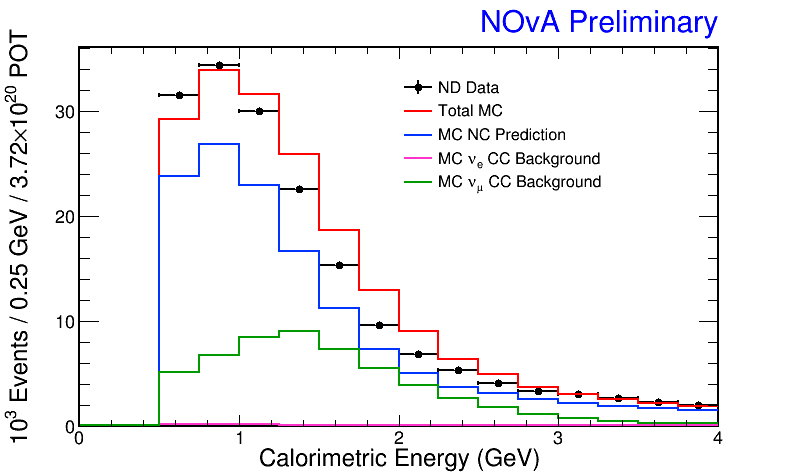
\includegraphics[width=.47\textwidth]{figures/DecompCheat.png} &
    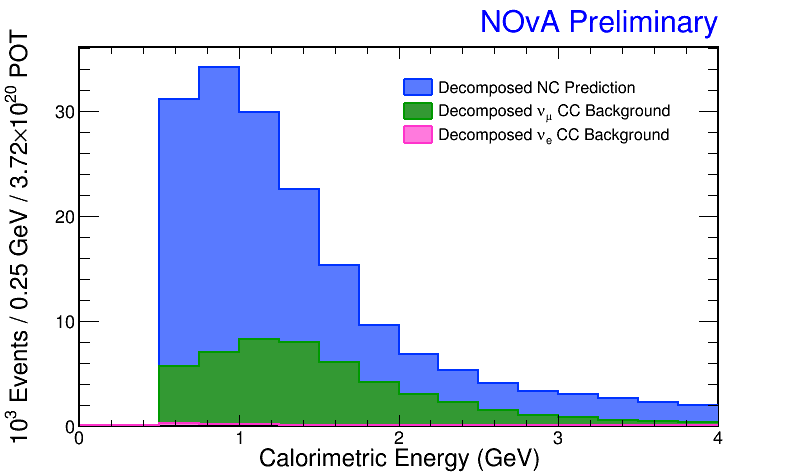
\includegraphics[width=.47\textwidth]{figures/DecompProp.png} \\
  \end{tabular}
  \caption[ND Decomposition]{ND data decomposed into individual components. Left: the total data, total MC, and each MC component (not split by sign). Right: a stacked histogram of the decomposed data.}
  \label{fig:NDDecomp}
\end{figure}

\section{Extrapolation}
\label{sec:AnaExtrap}

The next part of the analysis chain extrapolates the ND data to the FD using both ND and FD MC. The output of the extrapolation is each oscillation component in bins of reconstructed energy (also called calorimetric energy) and true energy. The advantage of applying oscillation weights at a separate, later stage is that the extrapolation does not need to be repeated when applying many different oscillations as in a fit. There are two main types of extrapolations, indirect and direct. Indirect extrapolation involves measuring the ND data spectrum and using the data to tune the MC simulation. Direct extrapolation applies MC techniques to the measured ND spectra. For the analysis presented here, a simple Far Over Near (F/N) direct extrapolation method was used. 

The basic premise of the extrapolation is to apply a F/N ratio to the data.
\beq
\mbox{FD}^{Pred} = \mbox{ND}^{Data} \frac{\mbox{FD}^{MC}}{\mbox{ND}^{MC}} = \mbox{FD}^{MC} \frac{\mbox{ND}^{Data}}{\mbox{ND}^{MC}}
\label{eq:ExtrapFN}
\eeq

\n This method takes advantage of the fact that systematic effects cancel to first order due to the use of functionally identical detectors. Consequently, the F/N ratio mainly encodes the differences between the two detector spectra due to flux kinematics. Note that the F/N ratio is equivalent to applying a ND data/MC ratio to the FD MC, as shown in the second equality of equation \ref{eq:ExtrapFN}.

The actual process is a bit more complicated than this, and the results depend on which variable the F/N ratio in and what selection cuts are applied at the ND. For components with with sufficient statistics and energy resolution, the F/N ratio can be applied in bins of true energy. This requires more MC information and extra error checking. As the statistics or energy resolution degrades, the F/N ratio is applied only in bins of calorimetric energy. For the components with the least information, the FD MC is taken as the component prediction. Each component is extrapolated separately using one of these three methods. For appearance components, $\nu_\alpha \rightarrow \nu_\beta$, it is important to apply a $\nu_\alpha$-like selection to the ND spectra. This provides the most accurate correction to the FD MC as can be seen from the ND data/MC interpretation of equation \ref{eq:ExtrapFN}. Of course, the desired output is a number of events selected as NC-like, so the NC selection cuts are always applied at the FD.

The goal of the extrapolation is to predict the number of events from each component that are selected as NC-like in bins of true and calorimetric energy, $\mbox{FD}^{Pred}_{\alpha\rightarrow\beta}(S_{NC}; E^R_i, E^T_j)$, where $S_x$ denotes $x$-like event selection, $E^R_i$ denotes the $i$th row of calorimetric energy, and $E^T_j$ denotes the $j$th row of true energy. This is represented as a two dimensional histogram. In the simplest case the MC is taken as the prediction,
\beq
\mbox{FD}^{Pred}_{\alpha\rightarrow\beta}(S_{NC}; E^R_i, E^T_j) = \mbox{FD}^{MC}_{\alpha\rightarrow\beta}(S_{NC}; E^R_i, E^T_j),
\label{eq:ExtrapNoRW}
\eeq

\n where $\mbox{FD}^{MC}$ denotes a quantity calculated from the MC. This method is used for the smallest CC background components with the lowest statistics, $\nuanu_\mu \rightarrow\,\nuanu_\tau$, $\nuanu_e \rightarrow\,\nuanu_\mu$, $\nuanu_e \rightarrow\,\nuanu_\tau$, $\anumu \rightarrow \anumu$, and $\anue \rightarrow \anue$. For components with better statistics, the FD MC is corrected in bins of calorimetric energy.
\beq
\mbox{FD}^{Pred}_{\alpha\rightarrow\beta}(S_{NC}; E^R_i, E^T_j) = \frac{ \mbox{FD}^{MC}_{\alpha\rightarrow\beta}(S_{NC}; E^R_i, E^T_j) \cdot \mbox{ND}^{Data}_\alpha (S_{NC}; E^R_i)}{\mbox{ND}^{MC}_\alpha (S_{NC}; E^R_i)}
\label{eq:ExtrapRecoRW}
\eeq

\n This method is used for the NC signal, $\numu$ and $\nue$ CC survival background components. All three of these are survival components $(\beta = \alpha)$ that have a directly comparable spectrum at the ND and FD, unlike with the appearance components, and this is why the NC event selection is applied to the ND spectra as well in equation \ref{eq:ExtrapRecoRW}. The remaining two components, $\nuanu_\mu \rightarrow\,\nuanu_e$, have enough ND statistics to apply the F/N ratio in bins of true energy. Since these are both appearance components from muon flavor neutrinos, a $\numu$-like event selection is applied at the ND, specifically the cut \verb|kNumuND| described in reference \cite{ref:TNNumuND}.
\beq
\mbox{FD}^{Pred}_{\alpha\rightarrow\beta}(S_{NC}; E^R_i, E^T_j) = \frac{ \mbox{FD}^{MC}_{\alpha\rightarrow\beta}(S_{NC}; E^R_i, E^T_j) \cdot \mbox{ND}^{Pred}_\alpha (S_{\numu}; E^T_j)}{\mbox{ND}^{MC}_\alpha (S_{\numu}; E^T_j)}
\label{eq:ExtrapTrueRW}
\eeq

\beq
\mbox{ND}^{Pred}_{\alpha}(S_{\numu}; E^T_j) = \sum_k \frac{ \mbox{ND}^{MC}_{\alpha}(S_{\numu}; E^R_k, E^T_j) \cdot \mbox{ND}^{Data}_\alpha (S_{\numu}; E^R_k)}{\mbox{ND}^{MC}_\alpha (S_{\numu}; E^R_k)}
\label{eq:ExtrapTrueND}
\eeq

\n Equation \ref{eq:ExtrapTrueND} can be interpreted as a two step process, where the combination of terms inside the sum normalizes the calorimetric energy columns to the data values, then sums across the true energy row to find the ND true energy predicted value. Equations \ref{eq:ExtrapRecoRW} and \ref{eq:ExtrapTrueRW} then have the same structure, where $\mbox{ND}^{Pred}$ is used as the data input. Note that for equations \ref{eq:ExtrapRecoRW}, \ref{eq:ExtrapTrueRW}, and \ref{eq:ExtrapTrueND}, if the $\mbox{ND}^{MC}$ value is $0$ the extrapolation falls back to using the base FD MC for the prediction, but only for the particular bin that would otherwise require division by $0$. Figure \ref{fig:FNRatio} shows the F/N ratio for the NC component, as well as the ND data/MC for the alternative interpretation of equation \ref{eq:ExtrapFN}. Figure \ref{fig:MCvsEX} shows how the extrapolation changes the predicted distribution of the NC component.
\begin{figure}[htb]
  \centering
  \begin{tabular}{c c}
    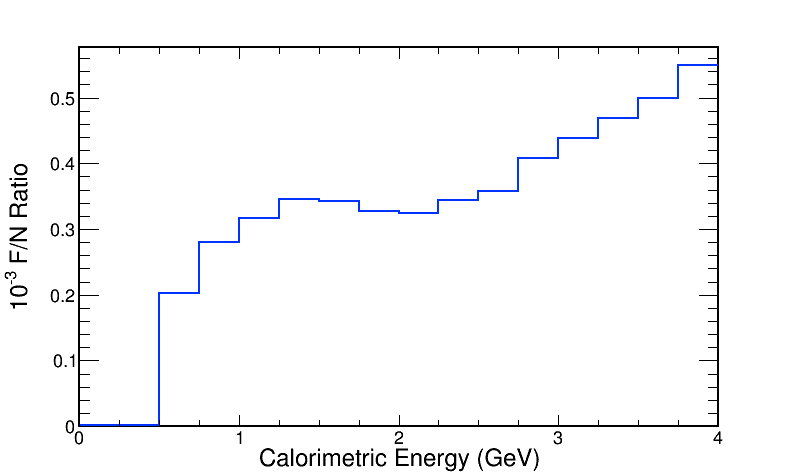
\includegraphics[width=.47\textwidth]{figures/Extrap/FNRatio.png} &
    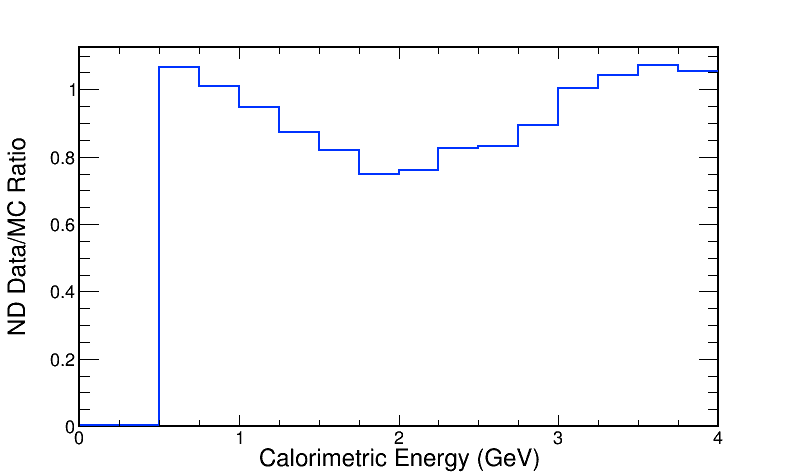
\includegraphics[width=.47\textwidth]{figures/Extrap/NDDatMC.png} \\
  \end{tabular}
  \caption[F/N Ratio and ND Data/MC Ratio for NC Component Extrapolation]{The left figure shows the F/N ratio for the NC component extrapolation. Equation \ref{eq:ExtrapFN} can also be interpreted as applying a ND data/MC ratio to the FD MC; this ratio is shown in the right figure.}
  \label{fig:FNRatio}
\end{figure}

\begin{figure}[htb]
  \centering
  \begin{tabular}{c c}
    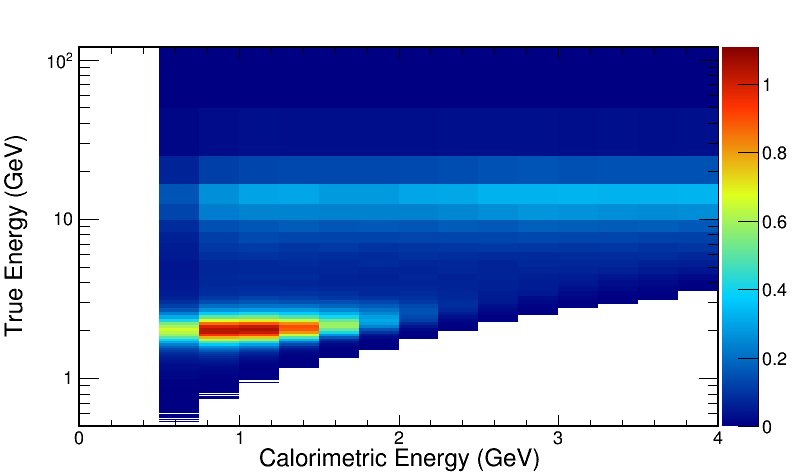
\includegraphics[width=.47\textwidth]{figures/Extrap/FDMC.png} &
    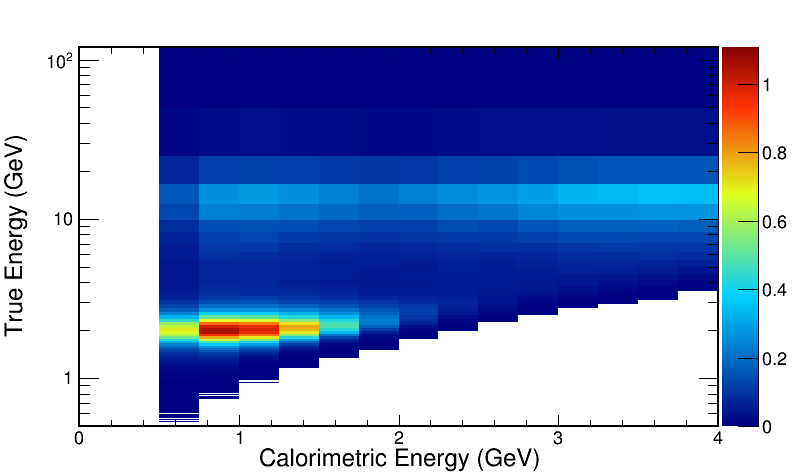
\includegraphics[width=.47\textwidth]{figures/Extrap/FDEX.png} \\
  \end{tabular}
  \caption[Effect of the Extrapolation on the NC Component Distribution]{These plots show how the extrapolation affects the predicted NC component distribution. Left: FD base MC. Right: Extrapolated spectrum. Both plots are scaled to \pot{6} and have the same Z axis range.}
  \label{fig:MCvsEX}
\end{figure}

In reality, only the neutrino flavor affects the oscillations, and not the interaction current. For the standard three flavor model, the number of NC interactions is not affected by oscillations, so it is okay to treat the NCs as any other component within the extrapolation. The NC disappearance analysis built its extrapolation upon the existing ModularExtrap class \cite{ref:TNModular} that handles the NC component in this fashion. However, when sterile neutrinos are added to the model, oscillations do affect the NC rate and thus the neutrino flavor breakdown of the NC interactions does matter. So long as the final neutrino flavor is an active one, the exact flavor does not matter. Therefore, it suffices to split the NCs based on their four initial flavors, $\nuanu_\mu$ and $\nuanu_e$. This was done by extrapolating the NCs as described above and splitting the FD result with flavor proportions constructed from the FD MC.
\beq
\mbox{FD}^{Pred}_{NC, \alpha}(S_{NC}; E^R_i, E^T_j) = \mbox{FD}^{Pred}_{NC}(S_{NC}; E^R_i, E^T_j) \frac{ \mbox{FD}^{MC}_{NC, \alpha}(S_{NC}; E^R_i) }{ \mbox{FD}^{MC}_{NC}(S_{NC}; E^R_i) }
\label{eq:ExtrapNCSplit}
\eeq

\n Figure \ref{fig:NCProportions} shows the flavor breakdown of the NC component. It was convenient to use this method based on what already existed within ModularExtrap, but it also avoided the need to construct raw spectra of the number of neutrinos per flavor using cross section information with large uncertainties.
\begin{figure}[htb]
  \centering
  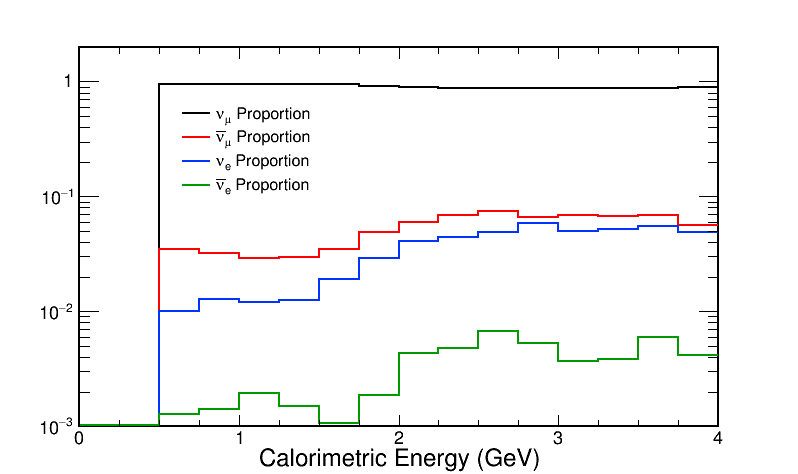
\includegraphics[width=.47\textwidth]{figures/Extrap/NCProportions.png}
  \caption[NC Component Flavor Proportions]{Proportions of the NC component from each neutrino flavor. The proportions are calculated based on the initial neutrino flavor, i.e., before oscillations are considered.}
  \label{fig:NCProportions}
\end{figure}

Table \ref{tab:ExtrapPred} summarizes the method used to extrapolate each component of the FD prediction.
\begin{table}[htb]
  \begin{center}
    \begin{tabular}{c c c c}
      \hline\hline
      Component & F/N Method & FD MC Prediction & Extrapolated Prediction \\
      \hline
      NC & Calorimetric Energy Bins & $65.19$ & $60.61$ \\
      $\numu \rightarrow\,\numu$ & Calorimetric Energy Bins & $4.98$ & $4.47$ \\
      $\numu \rightarrow\,\nue$ & True Energy Bins & $2.88$ & $2.83$ \\
      $\numu \rightarrow\,\nutau$ & Base FD MC & $0.32$ & $0.32$ \\
      $\anumu \rightarrow\,\anumu$ & Base FD MC & $0.10$ & $0.10$ \\
      $\anumu \rightarrow\,\anue$ & True Energy Bins & $0.043$ & $0.044$ \\
      $\anumu \rightarrow\,\anutau$ & Base FD MC & $0.046$ & $0.046$ \\
      $\nue \rightarrow\,\numu$ & Base FD MC & $0.010$ & $0.010$ \\
      $\nue \rightarrow\,\nue$ & Calorimetric Energy Bins & $0.77$ & $0.72$ \\
      $\nue \rightarrow\,\nutau$ & Base FD MC & $0.0010$ & $0.0010$ \\
      $\anue \rightarrow\,\anumu$ & Base FD MC & $0.0002$ & $0.0002$ \\
      $\anue \rightarrow\,\anue$ & Base FD MC & $0.036$ & $0.036$ \\
      $\anue \rightarrow\,\anutau$ & Base FD MC & $0.0001$ & $0.0001$ \\
      \hline
    \end{tabular}
    \caption[Extrapolation Method and Rate Summary]{Extrapolation method used for each component. The final two columns show the total number of predicted event rates after oscillations are applied as described in section \ref{sec:AnaPred}. These numbers used all diblock configurations and scaled to \pot{6.69} as described at the beginning of chapter \ref{ch:Results}. All components other than NC are CC backgrounds.}
    \label{tab:ExtrapPred}
  \end{center}
\end{table}

\section{Far Detector Prediction}
\label{sec:AnaPred}

Oscillations weights are applied in the final step of the analysis chain in the prediction step. The output of the extrapolation is required to contain true energy information as the oscillations are applied in bins of true energy. The predicted event spectrum for a given component is then calculated by summing over the bins of true energy, returning a one dimensional spectrum in calorimetric energy bins.
\beq
\mbox{FD}^{Pred}_{\alpha\rightarrow\beta}(S_{NC}; E^R_i) = \sum_j \mbox{FD}^{Pred}_{\alpha\rightarrow\beta}(S_{NC}; E^R_i, E^T_j) \cdot P(\nu_\alpha \rightarrow \nu_\beta, E^T_j)
\label{eq:PredComp}
\eeq

\n The NC component was handled as four separate components based on the initial neutrino flavor. For each of these, the probability of oscillating into any active neutrino flavor was applied.
\beq
\mbox{FD}^{Pred}_{NC, \alpha}(S_{NC}; E^R_i) = \sum_j \mbox{FD}^{Pred}_{NC, \alpha}(S_{NC}; E^R_i, E^T_j) \cdot P(\nu_\alpha \rightarrow \nu_{Active}, E^T_j)
\label{eq:PredNCComp}
\eeq
\beq
P(\nu_\alpha \rightarrow \nu_{Active}) \equiv \sum_{\ell \in \{e, \mu, \tau\}} P(\nu_\alpha \rightarrow \nu_\ell) = 1 - P(\nu_\alpha \rightarrow \nu_s)
\label{eq:PActive}
\eeq

\n The final event spectrum is simply the sum over all components, signal and background.
\beq
\mbox{FD}^{Pred}(S_{NC}; E^R_i) = \sum_{\{Comp\}} \mbox{FD}^{Pred}_{Comp}(S_{NC}; E^R_i)
\label{eq:Pred}
\eeq

The total event rates for each component, based on the oscillation parameters in table \ref{tab:3FlavParams}, are summarized in table \ref{tab:ExtrapPred}. This table also shows a comparison between the rates predicted by the base MC and the extrapolation. Figure \ref{fig:PredAllComp} shows all of the predicted component distributions based on the extrapolation, with the exception of cosmics.
\begin{figure}[htb]
  \centering
  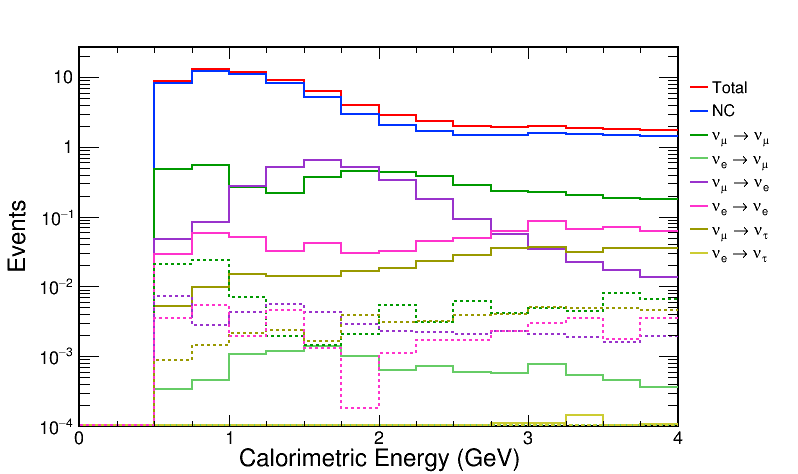
\includegraphics[width=.8\textwidth]{figures/FDPredAllComp.png}
  \caption[Predicted Component Distributions]{FD predicted distributions of all $13$ beam components, assuming oscillation parameters listed in table \ref{tab:3FlavParams}. The dashed line of a given color shows the predicted anti-neutrino component that corresponds to the component listed in the legend.}
  \label{fig:PredAllComp}
\end{figure}